\chapter{Electro-optical topology optimization problems}\label{chap:eo}
%\section{Electro-optical systems~\cite{ownpub4}}\label{sec:electro_optical}
Electro-optics describes the interaction between electricity and optics. Electricity involves the presence and flow of electric charges, which can generate electromagnetic fields.
However, the main difference is that the frequency of the electrical fields ($\omega_E$)
is much lower than for optical fields ($\omega_E \ll \omega $), so that they can be considered as static fields\footnote{Similarly, as discussed in \secref{sec:nanophotonics}, the size ($s$) of optical devices
is usually much smaller than the wavelength of the electrical fields ($s\ll \lambda_E $), so that the field is effectively quasistatic.}.
The interaction between electricity and optics is used in a variety of technologies such as high-speed modulators for optical communications~\cite{modu, modu1, modu2, pockels}, switches\cite{eo_switch}, electrically pumped lasers\cite{laser,laser_pic}, and integrated photonic circuits\cite{laser_pic}. 
These systems exploit mechanisms ranging from the electro-optic effect~\cite{eo_effect} to carrier-induced refractive index
 changes \cite{c_i_n} to achieve efficient light manipulation and generation, bridging electro-optic principles with carrier-driven processes central to optoelectronics.



As a basic example of electro-optic coupling one can consider the \textbf{electro-optic effect}~\cite{eo_effect} (analogous to the thermo-optic effect),
where the refractive index of a material can be modified under the influence of an external (static) electric field. The linear term in the electro-optic effect is known as the
Pockels effect~\cite{pockels} $
    \Delta n = -(1/2) n^3 r E\,,$
where $r$ is the electro-optic coefficient, and $E$ is the applied electric field. The quadratic term 
is known as the electro-optic Kerr effect $\Delta n = n_2 E^2$, where $n_2$ is the Kerr-coefficient~\cite{phot_crys}. Note based on the applied external
quasistatic electric field, one can model the refractive index change by accounting for higher order terms in the expansion of the polarizability
in terms of the electric field (\eqref{eq:polarization}), where the Pockels effect corrresponds to the $\chi^{(2)}$ term, and the Kerr effect to the $\chi^{(3)}$ term.

Building on this understanding of electro-optic phenomena, topology optimization has been extensively applied to design coupled electrical systems such as MEMS devices~\cite{MEMS_multi}, electrochemical systems~\cite{electrode}, and electrostatic actuators~\cite{electrostatic_act}. However, the field of electro-optics is
still relatively unexplored with few works, such as \cite{g_heat}, which studies the design of diffusion-based systems with applications on
carrier dynamics in semiconductor devices.

In the remainder of the section we focus on our work~\cite{ownpub4} , where we apply topology 
optimization to design a nanolaser device, where electrical pumping can be used to achieve efficient light emission.

\section{Topology optimization of nanolasers~\cite{ownpub4}}\label{sec:laser}

\subsection*{A Figure of Merit for nanolaser performance}

A nanolaser is a nanoscale laser device that emits light by stimulating the emission of photons in a gain medium, typically a semiconductor material. This is illustrated
in \figref{fig:laser2d}, where a pump laser excites the emitters/carriers (e.g., electrons and holes) in a gain medium $D_0$, which then emits light into an output channel (e.g., waveguide) via
stimulated emission. This physical
mechanism can be described by using the Maxwell-Bloch equations~\cite{haken_laser_dynamics, PhysRev.134.A1429, SALT_original}, which are a set of nonlinear time-dependent 
partial differential equations. When aligned to high-$Q$ ($Q\gtrapprox 100$~\cite{cerjan_2016}) lasing
mode, the system can be described via the single-pole approximation (SPA-) steady-state ab-initio laser theory (SALT)~\cite{Ge_2010}
\begin{equation}\label{eq:SPA_SALT}
    {\left[(\nabla \times 
     \nabla \times ) -\left(\varepsilon_c(\mathbf{r})-i \Delta \varepsilon^{\prime \prime} (\mathbf{r})\right) \left(\frac{\omega_L}{c}\right)^2\right] \mathbf{E}_L(\mathbf{r})=0}\,.
\end{equation}
where $\mathbf{E}_L$ is the lasing mode, $\omega_L$ is the lasing frequency, $\varepsilon_c$ is the dielectric permittivity of the passive (without gain) cavity, and the change in the 
imaginary part of the permittivity is given by
\begin{equation}\label{eq:gain_SALT}
        \Delta \varepsilon^{\prime \prime} (\mathbf{r}) =  \frac{D_0(\mathbf{r}) d}{1+ e_c^{-2}\left|\mathbf{E}_L(\mathbf{r})\right|^2}\,.
\end{equation}
where $D_0(\mathbf{r})$ is the gain profile, $d$ is a scalar pumping strength, and $e_c$ is a non-dimensionalization parameter~\cite{Ge_2010}. Although much simpler than the Maxwell-Bloch equations, \eqref{eq:SPA_SALT} still
requires one to solve a nonlinear eigenproblem, which can be computationally expensive, especially in inverse design problems where one needs to solve hundreds or thousands of these problems to optimize the device.

\begin{figure}[tb]
    \centering
    \makebox[\textwidth][c]{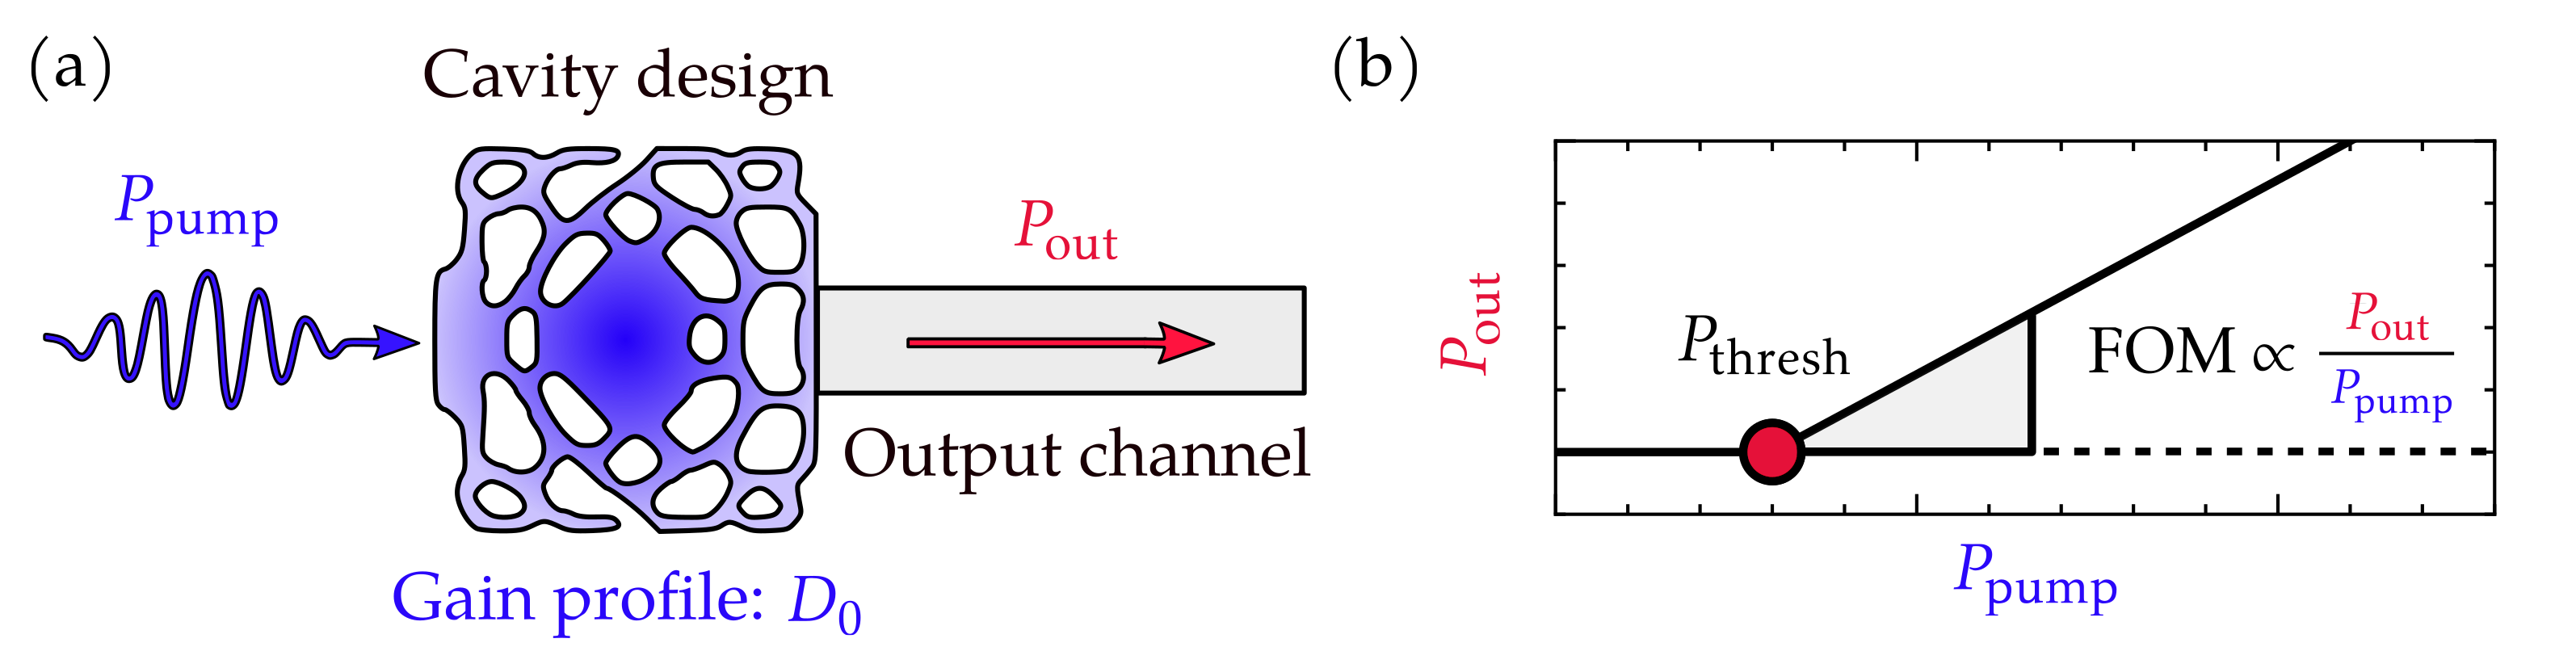
\includegraphics{figures/laser.png}}%%
    \caption{Topology optimization of nanolasers. (a) Working principle of a nanolaser. A pump power ($P_\text{pump}$) excites a a gain medium with profile
    $D_0$ that emits a single lasing mode into an output channel with power $P_\text{out}$. (b) The optimization FOM is proportional to the linear relation between the pump and output power ($P_\text{out}/P_\text{pump}$),
    just above the lasing threshold ($P \gtrapprox P_\text{thres}$).  Adapted from~\cite{ownpub4}.}
    \label{fig:laser2d}
\end{figure}

To circumvent this, in~\cite{ownpub4} we propose a synthesis of SPA-SALT, perturbation theory, and coupled mode theory to simplify the problem. 
The two key results of this derivation are the expression of the lasing threshold and the FOM for the optimization that can be evaluated by solving a linear system of equations.
One of the two key results derived from this framework is the expression for the \textbf{lasing threshold}~\cite{ownpub4} CHANGE GAMMA FACTOR THING
\begin{equation}\label{eq:pump_thresh}
    d_\text{thresh} = \frac{1}{\Gamma Q} = \frac{1}{Q} \frac{\int_{\Omega} \varepsilon_c(\mathbf{r})|\mathbf{E}_{\text{r}}(\mathbf{r})|^2\,  \d \Omega}{\int_{\Omega} D_0(\mathbf{r}) |\mathbf{E}_{\text{r}}(\mathbf{r})|^2\,  \d \Omega}\,.
\end{equation}
where $\mathbf{E}_\text{r}$ is the field in a reciprocal problem (\secref{sec:nanophotonics}) where the system is excited from an output port\footnote{In a high-$Q$ system, the field from the reciprocal solve $\mathbf{E}_r$ is almost exactly equal to the cavity mode plus a $\mathcal{O}(1/\sqrt{Q})$ error~\cite{phot_crys}.} (e.g. the waveguide in \figref{fig:laser2d}), $Q$ is the quality factor of the cavity resonance, and $\Gamma$ is a measure 
of energy confinement in the gain region. From this expression we see that one can reduce the lasing threshold (for more energy-efficient lasers) by increasing $Q$ and by enhancing the energy confinement in the
active medium ($\Gamma$). Note that in the single-emitter limit, where $D_0(\mathbf{r})\propto \delta (\mathbf{r}-\mathbf{r^\prime})$ for an emitter located at $\mathbf{r}^\prime$, this expression becomes $d_\text{thresh}=V/Q$, where $V$ is a measure
of the modal volume, a common FOM in other non-laser related inverse design works (e.g.,~\cite{LDOS_opt_wang}).

The second key result of the work is \textbf{a FOM for nanolaser design} (\secref{sec:nanophotonics}) that can also be evaluated through a single linear reciprocal solve~\cite{ownpub4}
\begin{equation}\label{eq:eff_nl}
    \frac{P_\text{out}}{P_\text{pump}} \propto \frac{\left( \int_{\Omega} D_0(\mathbf{r})|\mathbf{E}_{\text{r}}(\mathbf{r})|^2 \,  \d \Omega \right)^3} {\int_{\Omega} D_0(\mathbf{r}) |\mathbf{E}_{\text{r}}(\mathbf{r})|^4 \,  \d \Omega} = \text{FOM}.
\end{equation}
We will refer to this FOM as the \emph{nonlinear} FOM, since it accounts for the nanolaser nonlinearities perturbatively. The FOM is proportional to the laser efficiency ($P_\text{out}/P_\text{pump}$), and is roughly proportional 
to the energy in the cavity ($\sim |\mathbf{E}_{\text{r}}|^6 / |\mathbf{E}_{\text{r}}|^4 \sim |\mathbf{E}_{\text{r}}|^2$), and thus to the $Q$ factor, also contributing to a low
laser threshold (\eqref{eq:pump_thresh}). Thefore, as the optimization progresses the high-$Q$ assumption will become more and more accurate. In the single emitter limit the FOM becomes
$\text{FOM}=\vert \mathbf{E}_{r}(\mathbf{r}^\prime) \vert$, an
and LDOS-like FOM which via reciprocity is proportional to the total power emitted into an output channel~\cite[App.~C]{reci}. Note that this FOM also describes the case of a single-point gain region (e.g., a quantum dot),
whose location is randomly distributed in the cavity with a probability density $\mathcal{P} \sim D_0$. 

To show how the nonlinear FOM compares to more conventional cavity-optimization approaches, we introduce a “naive” generalization of the LDOS, which heuristically modifies the definition
of the LDOS to account for out-coupling efficiency (through a reciprocal solve $\mathbf{E}_r$) and a distributed gain
medium $D_0$
\begin{equation}\label{eq:SEL}
    \text{FOM}_{\text {naive }}=\int_{\Omega} D_0(\mathbf{r})\left|\mathbf{E}_{\text{r}}(\mathbf{r})\right|^2 \d \Omega
\end{equation}
which we refer to as the \emph{naive} FOM, defined by the overlap of the electric-field intensity of the reciprocal field with the gain distribution.
Note that this naive FOM is also proportional to the intensity of the reciprocal field ($\sim |\mathbf{E}_{\text{r}}|^2$), and thus roughly proportional to $Q$, thus ensuring 
high-$Q$ optimized cavities.

\subsection*{Optimization results for extended gain media}

\begin{figure}[tb]
    \centering
    \makebox[\textwidth][c]{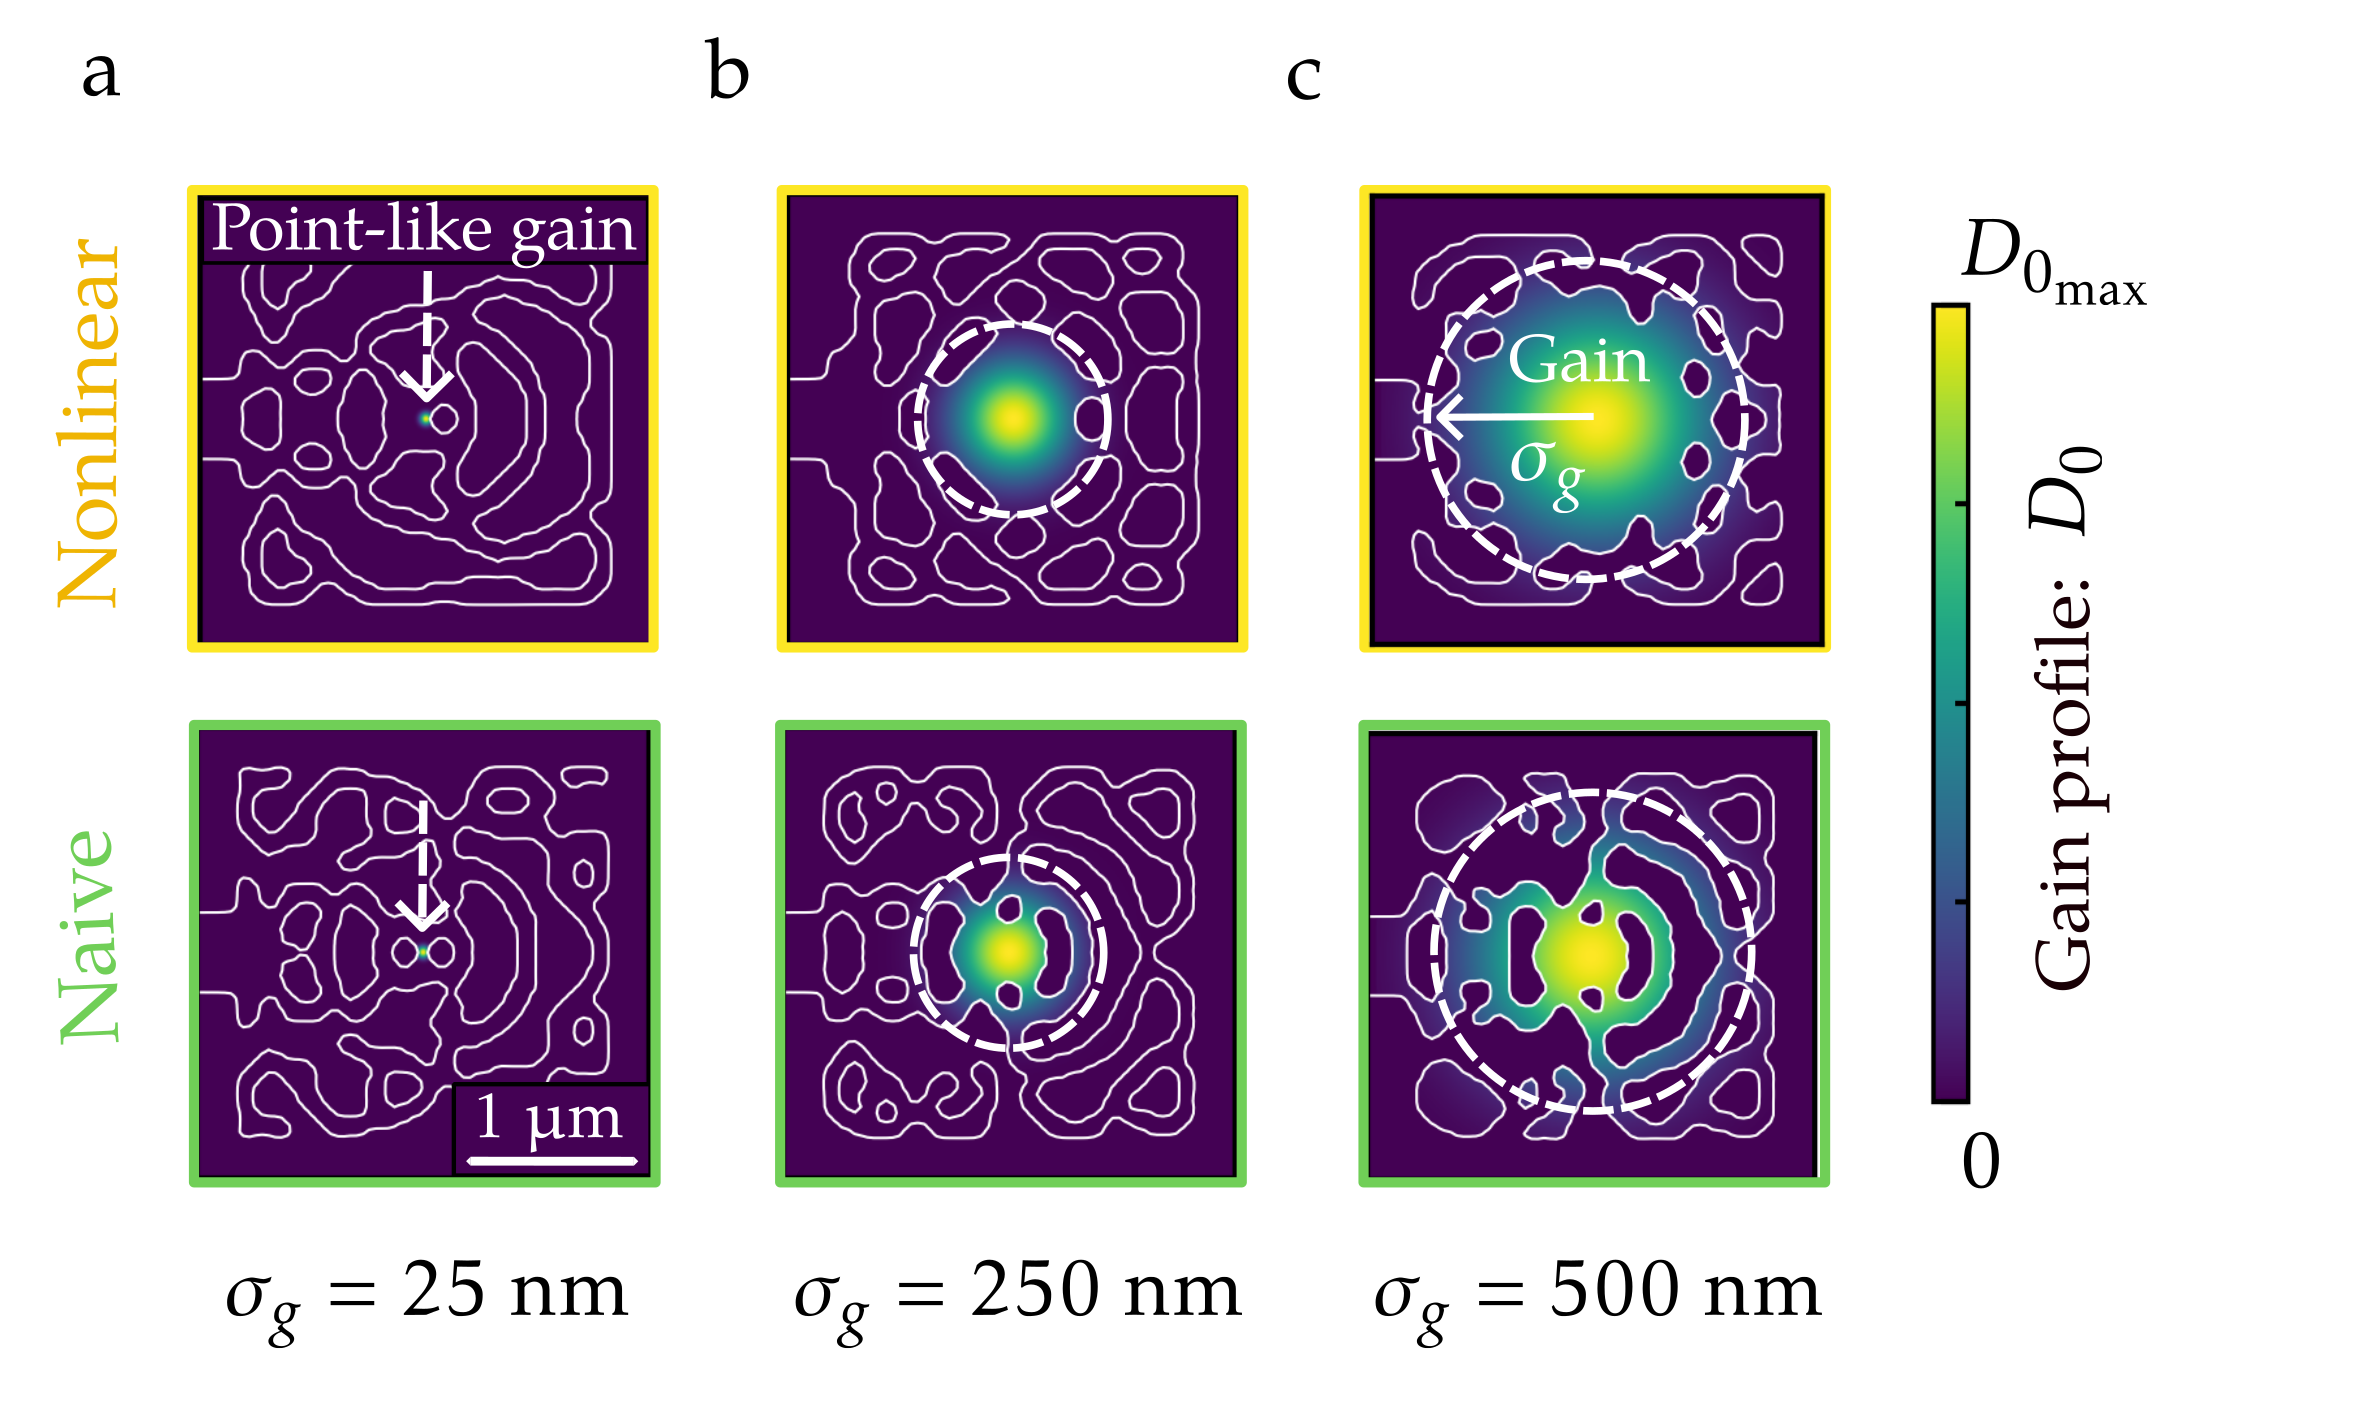
\includegraphics{figures/laser_size.png}}%%
    \caption{Performance of the topology-optimized devices for the nonlinear and naive FOMs for different Gaussian gain distributions with standard deviations $\sigma_g$. (a) Device optimize for a point-like gain region ($\sigma_g=25$ nm).
    (b) Device optimized for $\sigma_g=250$ nm. (c) Device optimized for $\sigma_g=500$ nm. Adapted from~\cite{ownpub4}.}
    \label{fig:laser_size}
\end{figure}

Appplying this formalism we optimize two-dimensional nanolasers, where we study the effect of the gain region size in 
nanolaser design (\figref{fig:laser_size}), and verify that for point-like gain regions the devices optimized for the FOM and the naive FOM (\eqref{eq:SEL})
achieve similar performance (limited by the finite size of the tiny gain region), favoring bowtie-like cavity designs
where the in-plane electric field can be concentrated at a bowtie sharpness-limited field singularity~\cite{sing}. Moreover, we show that for
larger distributed gain media the derived FOM discourages field localization due to the denominator in \eqref{eq:eff_nl} (since $\int \vert \mathbf{E} \vert^2$ is finite), in contrast to the naive FOM, 
resulting in a $\approx 3\times$ enhancement when targeting the correct nanolaser FOM (\eqref{eq:eff_nl}). 
\subsection*{Accounting for gain diffusion}

In semiconductors with extended gain media, it is essential to model the electrical effect of \textbf{carrier diffusion}. This effect can be introduced by modeling the semiconductor gain medium in the free-carrier approximation\footnote{Neglecting carrier-carrier Coulomb interactions.}, using a difussion 
equation~\cite{csalt}. Using this formalism we re-derive the expressionin for the lasing threshold (\eqref{eq:pump_thresh}) when accounting for carrier diffusion~\cite{ownpub4}, where the lasing threshold is
\begin{equation}\label{eq:pump_thresh_diff}
    d_\text{thresh} = \frac{1}{Q} \frac{\int_{\Omega} \varepsilon_c(\mathbf{r})|\mathbf{E}_{\text{m}}(\mathbf{r})|^2\,  \d \Omega}{\int_{\Omega} \mathbb{S} [D_0] (\mathbf{r}) |\mathbf{E}_{\text{m}}(\mathbf{r})|^2\,  \d \Omega}\,,
\end{equation}
and the nanolaser FOM (\eqref{eq:eff_nl}) with carrier diffusion effects
\begin{equation}\label{eq:eff_diff}
    \text{FOM} =  \frac{\left(\int_{\Omega} \mathbb{S} [D_0](\mathbf{r}) |\mathbf{E}_{\text{r}}(\mathbf{r})|^2 \,  \d \Omega\right)^3} {\int_{\Omega} \mathbb{S}\left[ |\mathbf{E}_{\text{r}}|^2\, \mathbb{S} [D_0] \right] (\mathbf{r})|\mathbf{E}_{\text{r}}(\mathbf{r})|^2 \,  \d \Omega}\,.
\end{equation}
These expressons use the diffusion operator $\mathbb{S}^{-1}= \mathbb{I}+\nabla \cdot (R_\nabla^2(\mathbf{r}) \nabla)$, where $\mathbb{I}$ is the identity operator, and $R_\nabla (\mathbf{r})$ is a diffusion lengthscale determined by the spatially- and design-dependent diffusion coefficient combined with the damping/recombination rate. 
In this notation computing $u = \mathbb{S}[b]$ corresponds to solving for the scalar field $u$ in the diffusion problem $\mathbb{S}^{-1}u=b$, where $b$ is a scalar field. 
The difference when accounting for difussion is that now one needs to consider the profile of diffused carriers $\mathbb{S} [D_0]$ in the lasing threshold, and the diffusion of the gain depletion
in the FOM denominator. Note that in the small diffusion limit ($R_\nabla \ll \lambda, \mathbb{S} \approx \mathbb{I}$)
we recover the original expressions in \eqref{eq:pump_thresh} and \eqref{eq:eff_nl}.

\begin{figure}[tb]
    \centering
    \makebox[\textwidth][c]{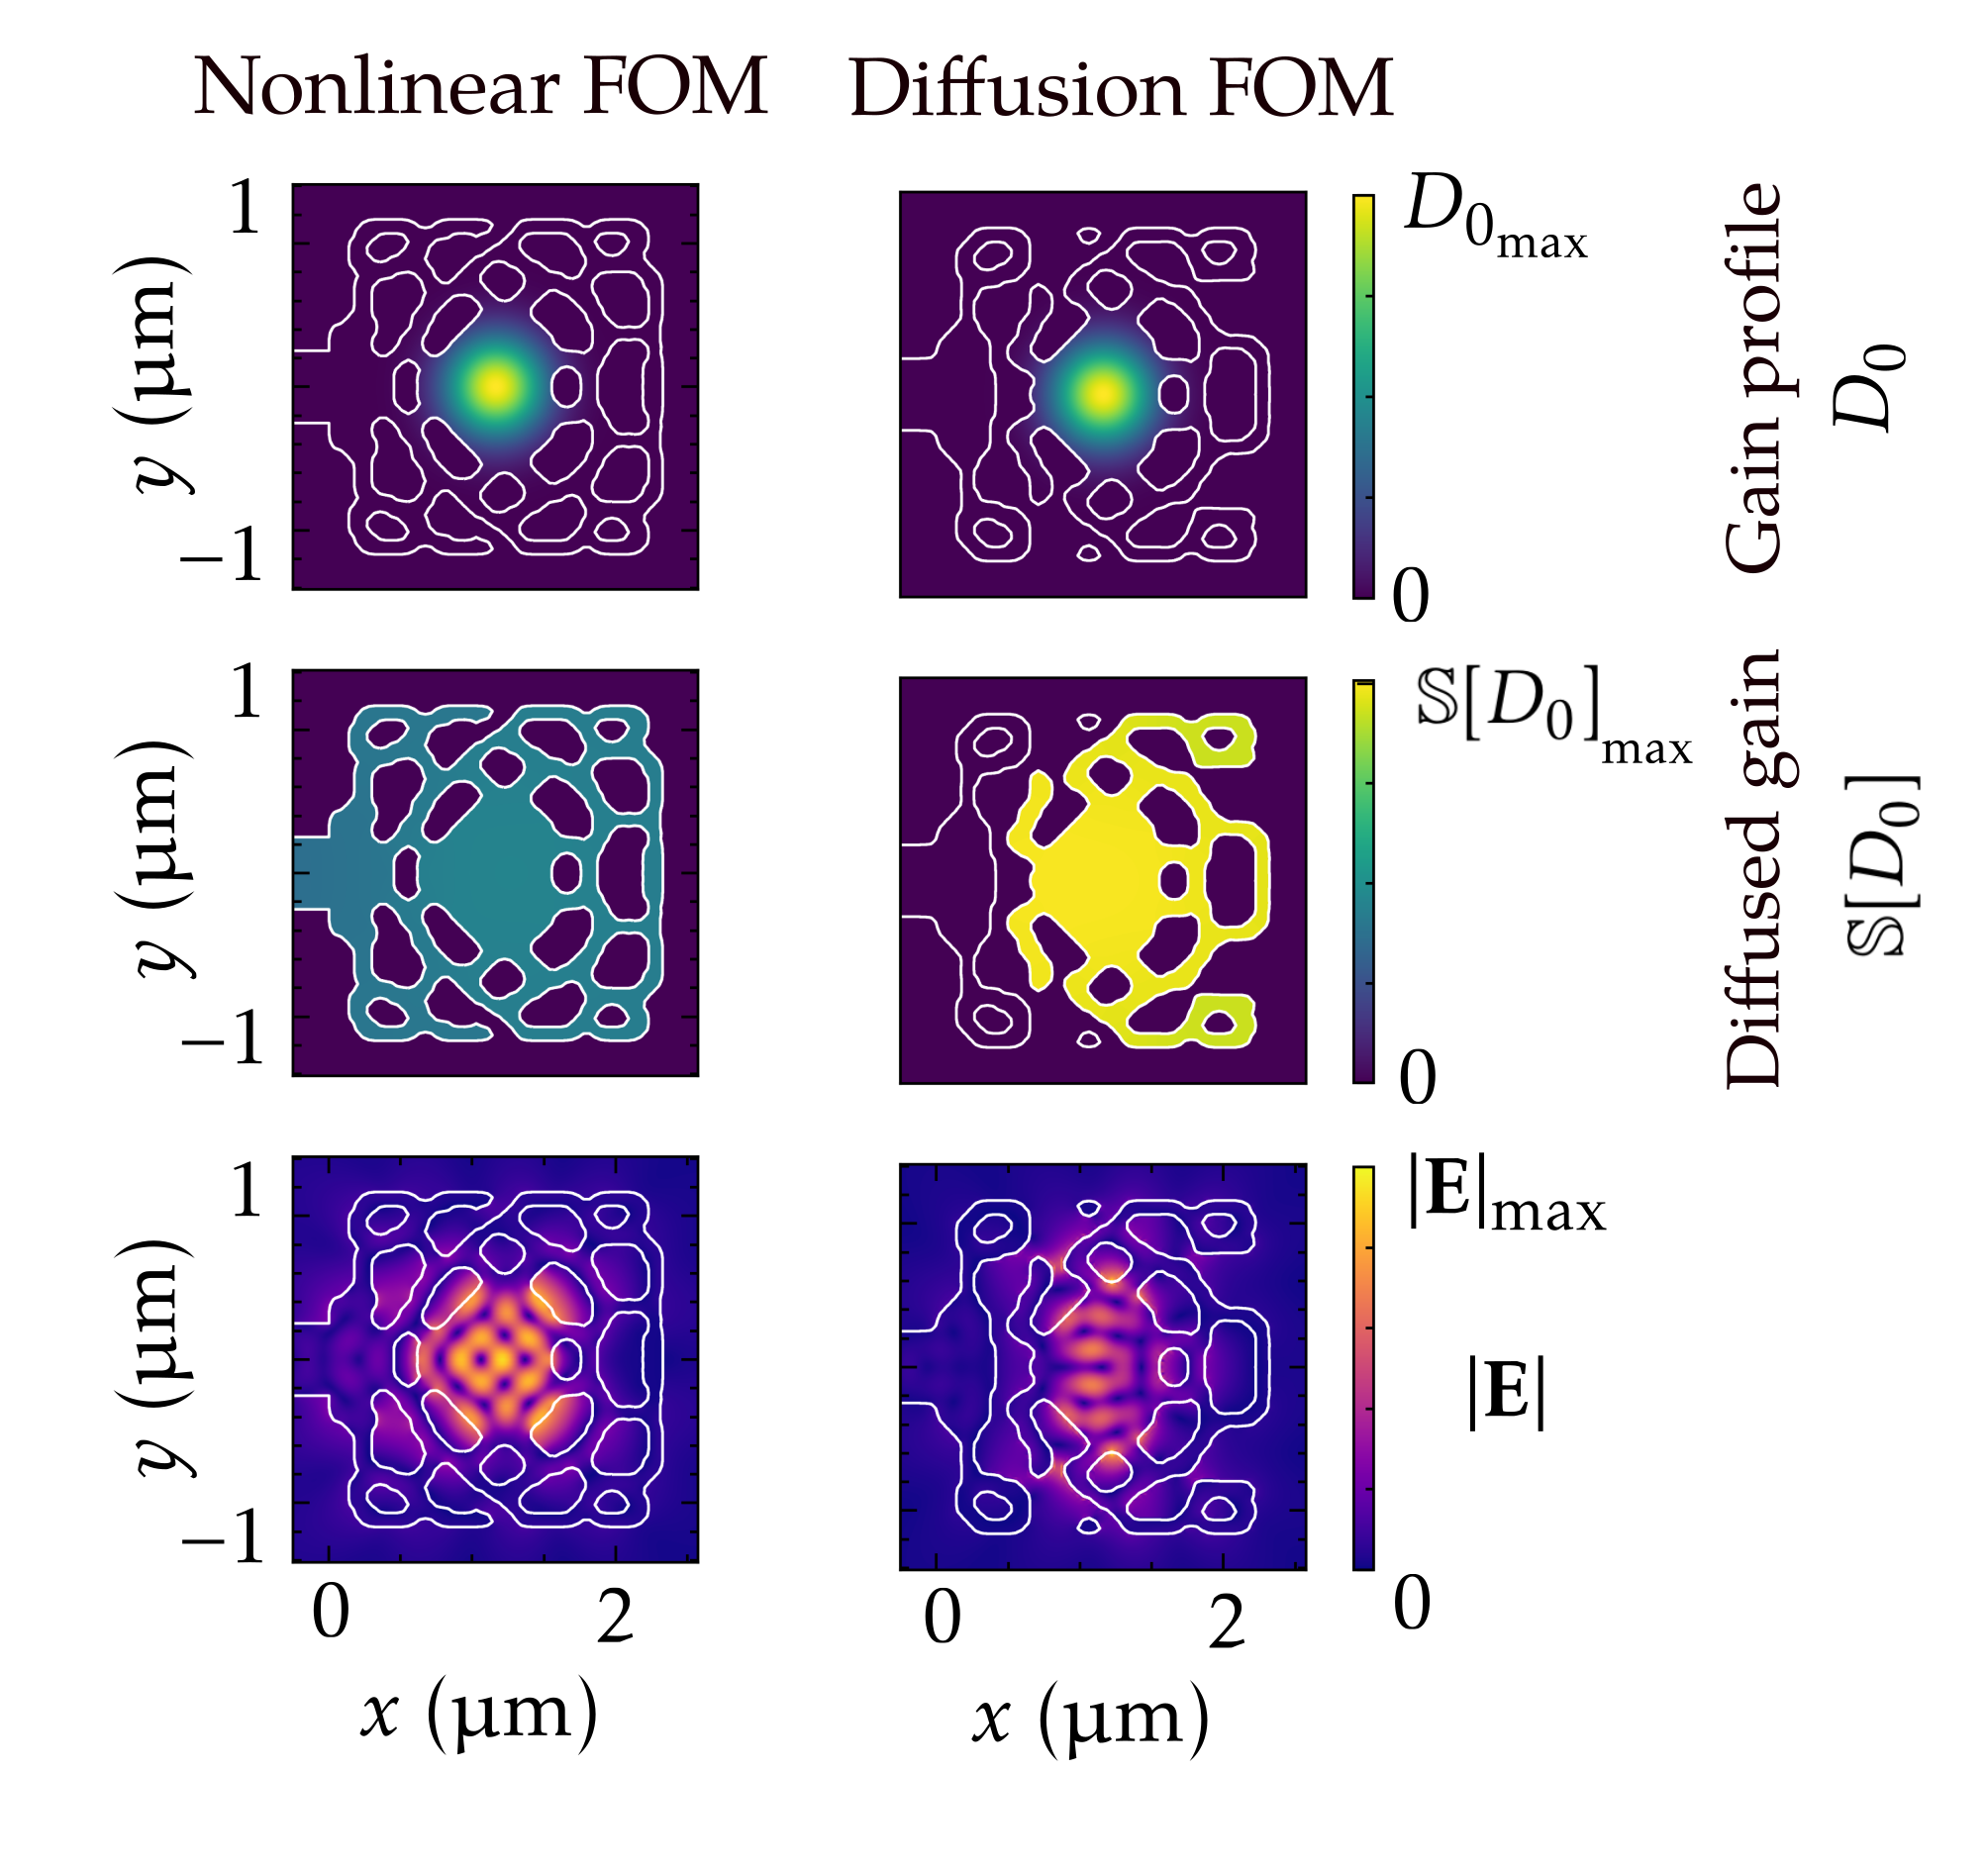
\includegraphics{figures/laser_carriers.png}}%%
    \caption{Topology-optimized devices with gain diffusion effects for a gain region with size $\sigma_g=250$ nm and a diffusion length of $R_\nabla=5$ \textmu m. The device optimized without accounting for gain diffusion ("Nonlinear FOM") and the device optimized accounting for gain diffusion ("Diffusion FOM") have the gain profile $D_0$ that is diffused ($\mathbb{S}[D_0]$)
    in the semiconductor-like material, generating the optical field given by the electric-field norm $\vert \mathbf{E} \vert$. Adapted from~\cite{ownpub4}.}
    \label{fig:laser_diff}
\end{figure}

By using the expression in \eqref{eq:eff_diff} as an optimization FOM, we study how accounting for diffusion effects
affects nanolaser designs and performance. As shown in \figref{fig:laser_diff}, the device that accounts for diffusion disconnects the cavity from the waveguide while also removing
material from areas of weak electric field, to 
enhance the coupling between the carriers and the optical field, and results in a $\approx 2\times$ enhancement when considering the diffusion-corrected FOM. 

\subsection*{Towards realizable nanolasers: three-dimensional designs}

Finally, we also apply the formalism to design three-dimensional silicon-on-insulator nanolasers (\figref{fig:laser3d}), 
and verify that similar to the two-dimensional case, the FOM discourages field localization while still efficiently coupling to the output waveguide, yielding a $\approx 1.6\times$
enhancement when considering the correct FOM for extended gain media. Note that the enhacement drop with respect to the two-dimensional optimization results
is attributed to the fact that localizing a high-$Q$ resonance is more difficult in three-dimensions.

\begin{figure}[tb]
    \centering
    \makebox[\textwidth][c]{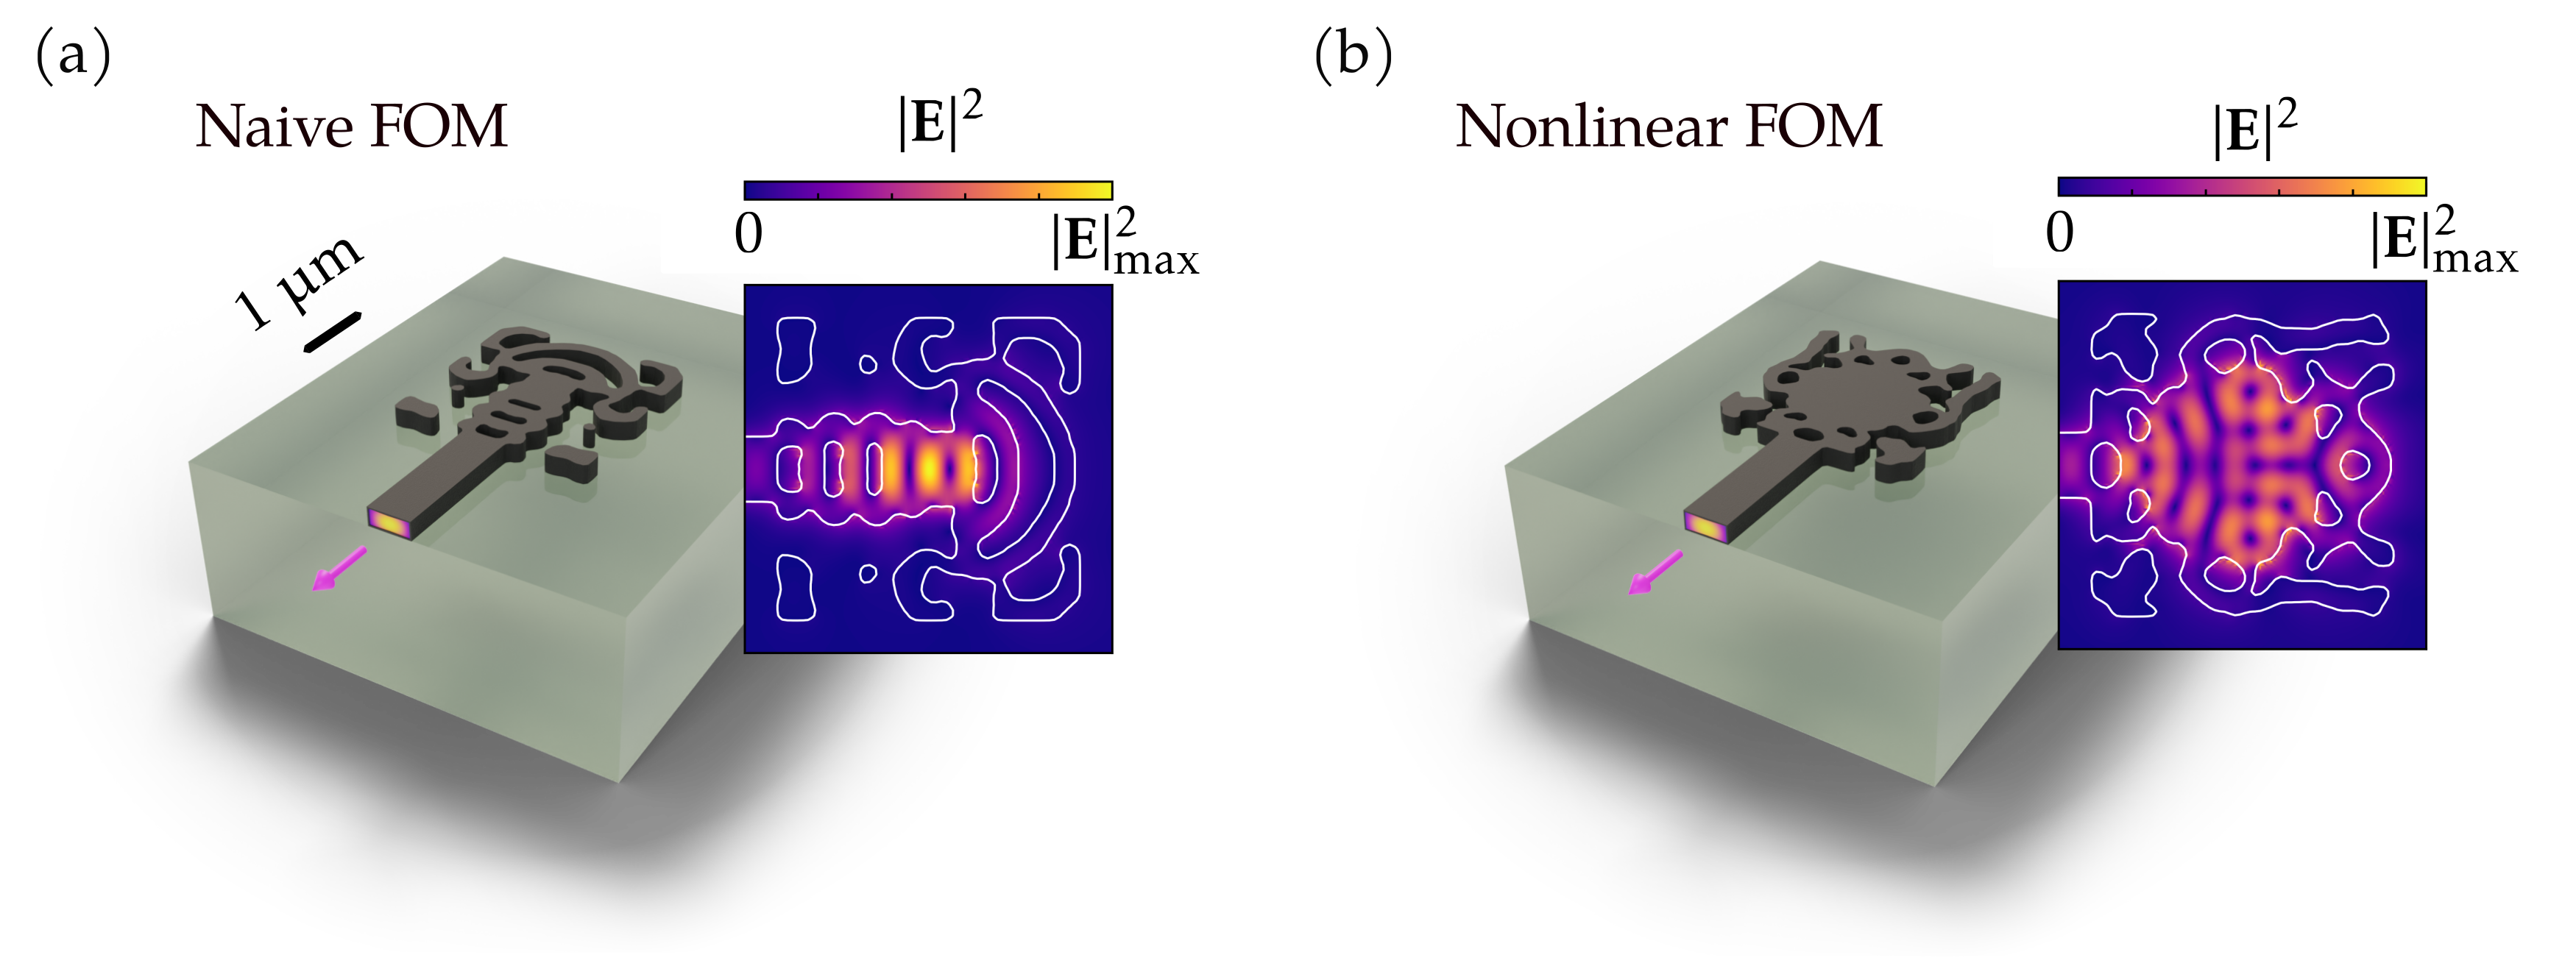
\includegraphics{figures/laser_2.png}}%%
    \caption{Topology-optimized nanolasers in three dimensions. The devices las into the cavity mode (inset plot) and out-couple to the waveguide mode. (a) Device optimized for the naive FOM. (b) Device optimized for the nonlinear FOM.
    Adapted from~\cite{ownpub4}.}
    \label{fig:laser3d}
\end{figure}

\subsection*{Outlook and future work}

In conclusion, in \cite{ownpub4} we show that by exploiting perturbative analysis valid in high-$Q$ cavities, one can derive  
an efficient FOM for laser performance ($\propto P_\text{out}/P_\text{pump}$) that captures resonant enhancement,  
spatial hole-burning, and gain diffusion at little extra computational cost. The FOM evaluation requires only a  
single linear reciprocal Maxwell solve (plus potentially two scalar solves for gain diffusion), making it 
an efficient formulation for laser optimization. This efficient first-principles approach allows for inverse nanolaser design in two and three dimensions, while  
also allowing for future refinements, including accounting for the laser linewidth~\cite{pick}, or accurate pumping models, where optical or electrical pumping could be explicitly
modeled.
